\documentclass{article}
\usepackage{geometry}
\geometry{a4paper, margin=1in}
\usepackage{amsmath}
\usepackage{graphicx}
\usepackage{hyperref}
\usepackage{float}

\title{ATOM12 homologové}
\author{Tomáš Jelínek}
\date{\today}

\begin{document}

\maketitle


\section*{Postup}

\subsection*{Blast}
\begin{enumerate}
\item V Uniprotu jsme si našel onu sequenci a blastnul ji.
    \begin{itemize}
        \item Výsledek: \url{https://www.uniprot.org/blast/uniprotkb/ncbiblast-R20241105-090514-0876-7530075-p1m/overview}
    \end{itemize}
\item Z taxonomie je vidět, že to nenašlo jen protisty, takže se musí vyhodit ty 2 bakterie a jedna houba.
\item Stáhnul jsem si \textit{.json} soubor toho blastu
\item Json jsem pomocí skriptu co už napsal někdy dávno převedl na fasta soubor (možná to jde lehčeji?)
\end{enumerate}

\begin{figure}[H]
    \centering
    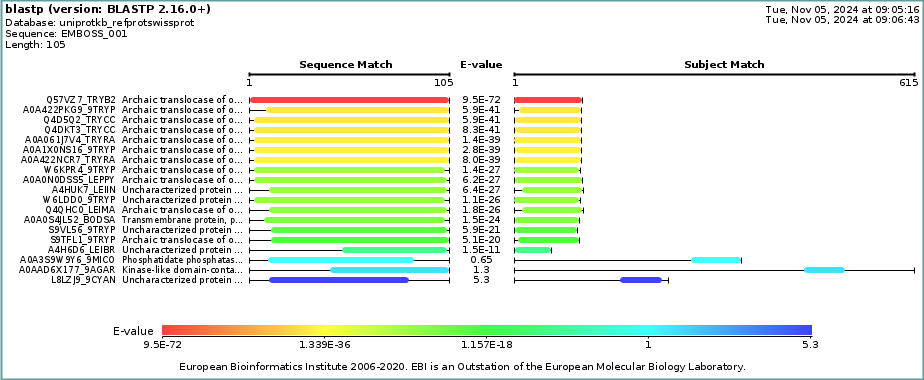
\includegraphics[width=0.8\textwidth]{vizualiazce.png}
    \caption{Je vidět, že ty bakterie a houba jsou na konci a dle E value i false positives prostě no}
    \label{fig:blast}
\end{figure}

\subsection*{MSA}

\begin{enumerate}
    \item MSA jsem udělal na .fasta souboru pomocí mého balíčku \href{https://github.com/Desperadus/PhyloBuilder}{PhyloBuilder}
    \item Zde jsou linky na joby: \href{http://www.ebi.ac.uk/jdispatcher/msa/clustalo/summary?jobId=clustalo-R20241105-161354-0975-92954007-p1m}{ClustalOmega}, \href{http://www.ebi.ac.uk/jdispatcher/msa/tcoffee/summary?jobId=tcoffee-R20241105-161452-0271-17506642-p1m}{tcoffee}, \href{http://www.ebi.ac.uk/jdispatcher/msa/muscle/summary?jobId=muscle-R20241105-161613-0467-63803921-p1m}{Muscle} 
    \item Tcoffee to udělal docela blbě
\end{enumerate}

\begin{figure}[H]
    \centering
    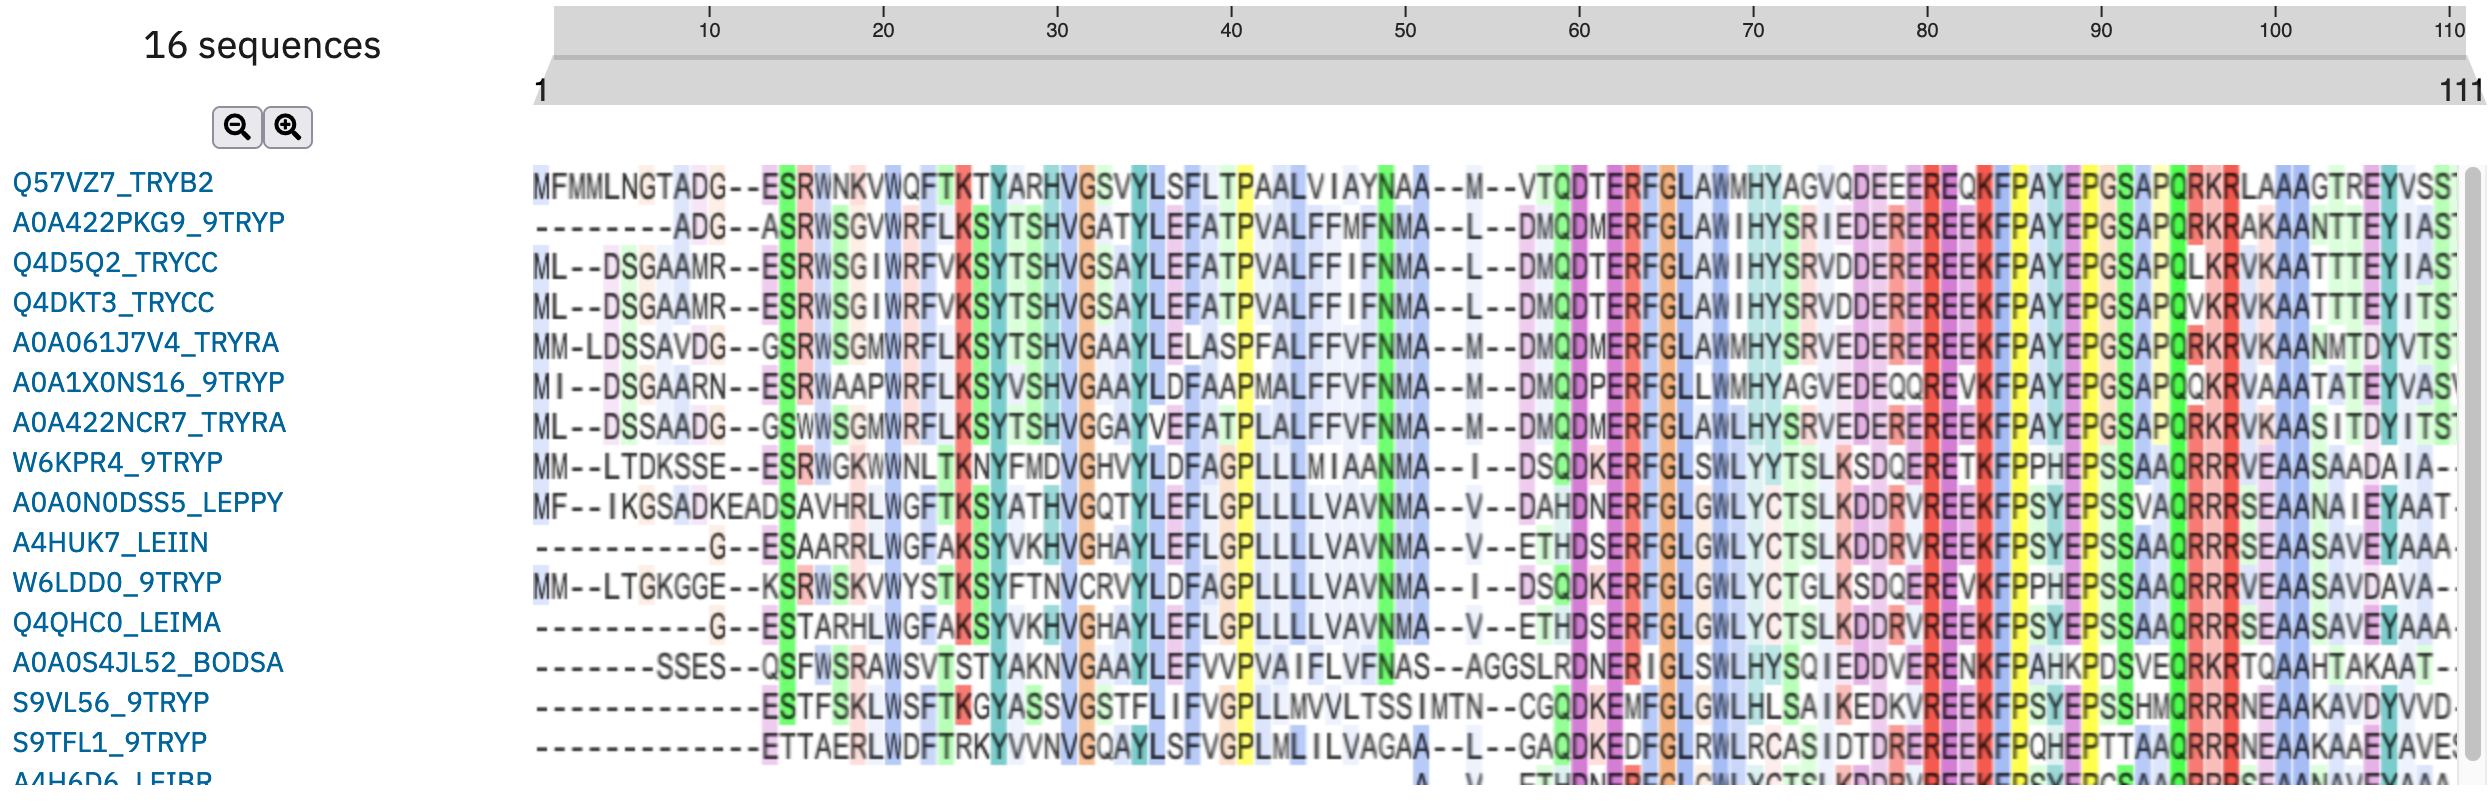
\includegraphics[width=0.8\textwidth]{tcoffee.png}
    \caption{Tcoffee}
\end{figure}

\begin{figure}[H]
    \centering
    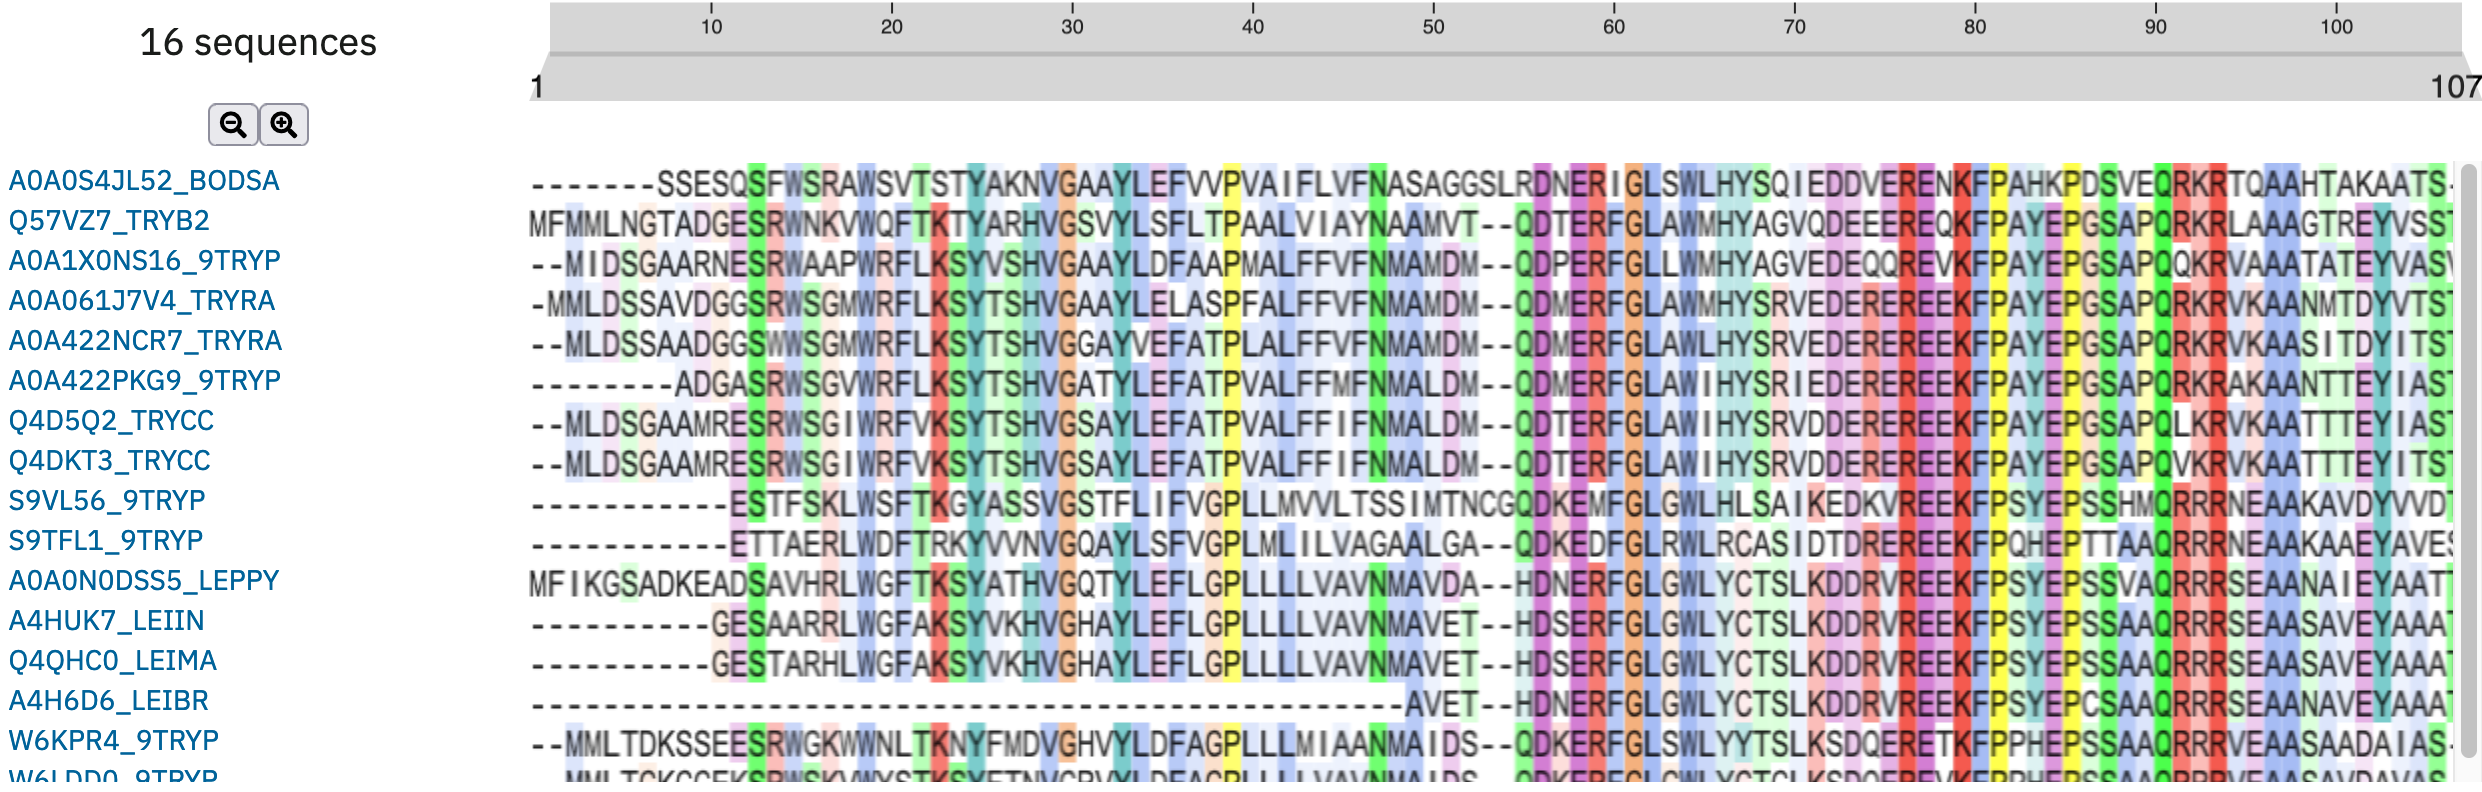
\includegraphics[width=0.8\textwidth]{muscle.png}
    \caption{Muscle}
\end{figure}

Upřímně moc nevím, kde tady hledat problémové části, přijde mi to docela v pohodě - když už, tak asi holt ten začátek a prostředek případně.


\end{document}